%%%%%%%%%%%%%%%%%%%%%%%%%%%%%%%%%%%%%%%%%%%%%%%%%%%%%%%%%%%%%%%%%%%%%%%%%%%%%%%%
\chapter{Περιγραφή Στερεών Σωμάτων}

Στο κεφάλαιο αυτό γίνεται μια σύντομη περιγραφή της μαθηματικής διατύπωσης του προβλήματος της κινηματικής και της δυναμικής των στερεών σωμάτων. Αρχικά μελετούνται οι σχετικοί μετασχηματισμοί, που είναι το βασικό εργαλείο περιγραφής της θέσης και του προσανατολισμού των σωμάτων. Έπειτα γίνεται μια σύντομη περιγραφή της κίνησης των σωμάτων από την σκοπιά των σχετικών μετασχηματισμών και περιγράφεται η διαδικασία της αντίστροφης κινηματικής. Τέλος, επεκτείνεται η ανάλυση στα προβλήματα της αντίστροφης και ορθής δυναμικής και προτείνονται τρόποι επίλυσης τους\footnote{Για περισσότερες πληροφορίες σχετικά με την μοντελοποίηση και την τυποποίηση των εξισώσεων ο αναγνώστης μπορεί να καταφύγει στα \cite{craig95, murray94}.}.

%%%%%%%%%%%%%%%%%%%%%%%%%%%%%%%%%%%%%%%%%%%%%%%%%%%%%%%%%%%%%%%%%%%%%%%%%%%%%%%%
\section{Μετασχηματισμοί}

Η θέση και ο προσανατολισμός ενός στερεού σώματος στο χώρο αναφορικά με ένα αδρανειακό καρτεσιανό πλαίσιο συντεταγμένων $\{Β\}$ γίνεται με την περιγραφή της θέσης και του προσανατολισμού ενός καρτεσιανού πλαισίου $\{Α\}$, το οποίο στερεώνουμε σε ένα αυθαίρετο σημείο του σώματος, π.χ. στο κέντρο μάζας. Το διάνυσμα θέσης του πλαισίου $\{Β\}$ εκφρασμένο στο αδρανειακό πλαίσιο $\{Α\}$ με $^AP_{BORG}$ και περιγράφει την θέση του στερεού σώματος ενώ ο πίνακας $^AR_B$ περιγράφει τον προσανατολισμό του σε σχέση με το αδρανειακό σύστημα. Το ζεύγος $\{^AP_{BORG}, ^AR_B\}$ περιγράφουν πλήρες την διάταξη του στερεού σε σχέση με το αδρανειακό \ref{fig:transformation}. Έτσι μπορεί κανείς να εκφράσει την σχετική θέση ενός σημείου στο πλαίσιο $\{Β\}$ ως προς το πλαίσιο  $\{Α\}$ ως εξής:

\begin{equation}
    ^AP = ^AT_B \cdot ^BP, \quad
    ^AT_B =
    \begin{bmatrix}
        ^AR_B & ^AP_{BORG}\\
        0 & 1
    \end{bmatrix}
\end{equation}

\begin{figure}[H]
    \centering
    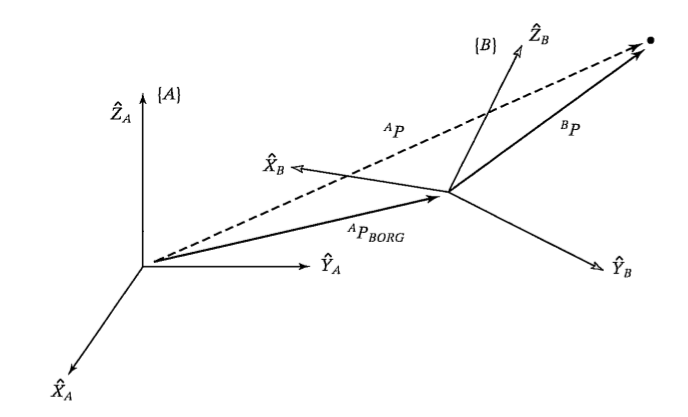
\includegraphics[width=.7\textwidth]{rigidbody/fig/transofrmation.png}
    \caption{Σχετικός μετασχηματισμός\protect\footnotemark}
    \label{fig:transformation}
\end{figure}
\footnotetext{Εικόνες από το βιβλίο \cite{craig95}}

Στις περιπτώσεις όπου έχουμε αλυσίδες από πλαίσια που ενώνονται με τους αντίστοιχους σχετικούς μετασχηματισμούς, μπορούμε να εκφράσουμε την σχετική θέση ενός πλαισίου πολλαπλασιάζοντας του αντίστοιχους μετασχηματισμούς. Όπως φαίνεται και στην εικόνα \ref{fig:transformation-chain} μπορεί να υπάρχουν εναλλακτικές διαδρομές που περιγράφουν την θέση ενός πλαισίου και οι μετασχηματισμοί που ισχύουν, μπορούν να περιγραφούν από τις εξισώσεις \ref{equ:chain}. Σε περίπτωση που υπάρχει κάποιος άγνωστος μετασχηματισμός, μπορεί κανείς να λύσει ως προς τον άγνωστο δοσμένου ότι γνωρίζει τους υπόλοιπους.

\begin{figure}[H]
    \centering
    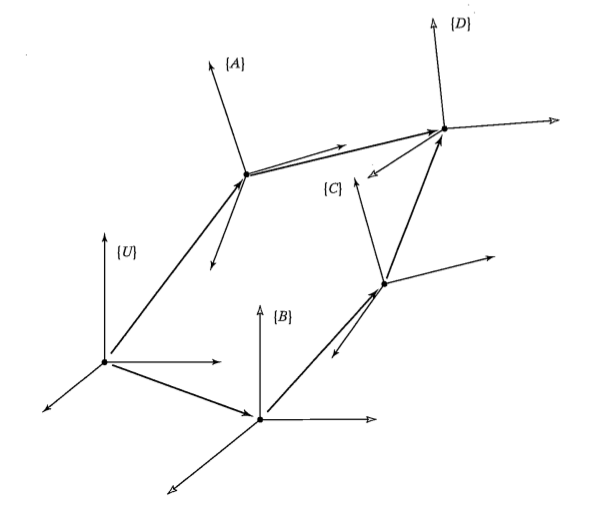
\includegraphics[width=.7\textwidth, height=.4\textheight]{rigidbody/fig/transformation-chain.png}
    \caption{Αλυσίδες μετασχηματισμού}
    \label{fig:transformation-chain}
\end{figure}

\begin{equation}
    \begin{aligned}
        ^UT_D = {}^UT_A \cdot {}^AT_D\\[10pt]
        ^UT_D = {}^UT_B \cdot {}^BT_C \cdot {}^CT_D\\[10pt]
        ^UT_A \cdot ^AT_D = {}^UT_B \cdot {}^BT_C \cdot {}^CT_D
    \end{aligned}
    \label{equ:chain}
\end{equation}

%%%%%%%%%%%%%%%%%%%%%%%%%%%%%%%%%%%%%%%%%%%%%%%%%%%%%%%%%%%%%%%%%%%%%%%%%%%%%%%%
\section{Κινηματική}

Για να κατανοήσουμε το πρόβλημα της κινηματικής, αλλά και της δυναμικής πρέπει να ξεκαθαριστεί η αλληλεπίδραση των ταχυτήτων σε ένα σύστημα στερεών σωμάτων. Για το λόγω αυτό πριν προχωρήσουμε στην ανάλυση απαιτείται μια μικρή εισαγωγή στο πως απορρέουν οι εξισώσεις που περιγράφουν την ταχύτητα ενός στερεού με χρήση των σχετικών μετασχηματισμών. Στην συνέχει θα γενικεύσουμε σε συστήματα σωμάτων.

%%%%%%%%%%%%%%%%%%%%%%%%%%%%%%%%%%%%%%%%%%%%%%%%%%%%%%%%%%%%%%%%%%%%%%%%%%%%%%%%
\subsection{Μελέτη της Ταχύτητας}

Έστω ότι θέλουμε να μελετήσουμε την κίνηση ενός σημείου $^BQ$ που ανήκει σε ένα στέρεο σώμα. Στην γενική περίπτωση, το σημείο θα έχει μια γραμμική ταχύτητα ως προς κάποιο πλαίσιο $\{Β\}$. Το πλαίσιο $\{Β\}$ θα έχει και αυτό γραμμική και περιστροφική ταχύτητα ως προς κάποιο πλαίσιο παρατήρησης, έστω $\{Α\}$. Θα θέλαμε να εκφράσουμε την ταχύτητα που έχει το σημείο $Q$ ως προς το πλαίσιο παρατήρησης όπως φαίνεται στην εικόνα \ref{fig:velocity}.

\begin{figure}[H]
    \centering
    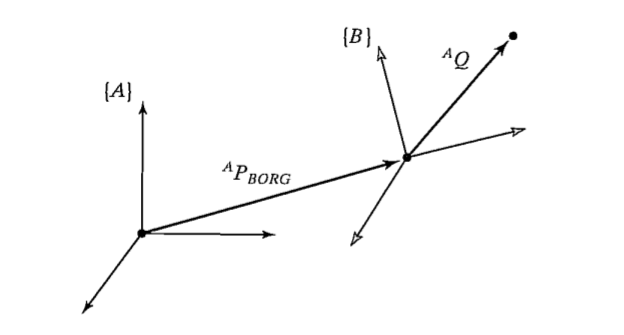
\includegraphics[width=.8\textwidth]{rigidbody/fig/velocity.png}
    \caption{Γενική περίπτωση κίνησης ενός σημείου\protect\footnotemark}
    \label{fig:velocity}
\end{figure}
\footnotetext{Εικόνα από το βιβλίο \cite{craig95}}

Έστω ότι η γραμμική ταχύτητα του πλαισίου $\{Β\}$ σε σχέση με το $\{Α\}$ είναι $^AV_{BORG}$ και η γωνιακή ταχύτητα είναι $^A\Omega_{BORG}$. Η γωνιακή ταχύτητα είναι ένα διάνυσμα, όπου η διεύθυνση εκφράζει τον άξονα περιστροφής, ενώ το μέτρο του την γωνία. Επίσης το σημείο $Q$ κινείται με ταχύτητα $^BV_Q$. Η γενική εξίσωση που περιγράφει την κίνηση του σημείου $Q$ δίνεται από την εξίσωση \ref{equ:q-velocity}.

\begin{equation}
    ^AV_Q = {}^AV_{BORG} + {}^AR_B \cdot {}^BV_Q + {}^A\Omega_B \times {}^AR_B
    \cdot {}^BQ
    \label{equ:q-velocity}
\end{equation}

Έστω ότι το σημείο $Q$ είναι αδρανειακό ως προς το πλαίσιο $\{Β\}$. Αν υποθέσουμε ότι το πλαίσιο παρατήρησης $\{Α\}$ συμπίπτει με το πλαίσιο $\{Β\}$, τότε η θέση του σημείου $Q$ ως προς το $\{Α\}$ δίνεται από την εξίσωση \ref{equ:position}.

\begin{equation}
    ^AQ = {}^AR_B \cdot {}^BQ
    \label{equ:position}
\end{equation}

Αν παραγωγίσουμε την σχέση \ref{equ:position} θα πάρουμε την ταχύτητα του σημείου ως προς το $\{Α\}$.

\begin{equation}
    \begin{split}
        ^A\dot{Q} & = {}^A\dot{R}_B \cdot {}^BQ\\
        ^AV_Q & = {}^A\dot{R}_B \cdot {}^AR^{-1}_B \cdot {}^AQ\\
        ^AV_Q & = {}^AS_B \cdot {}^AQ
    \end{split}
    \label{equ:velocity}
\end{equation}

Όπου $^AS_B$ είναι ο αντισυμμετρικός πίνακας και εκφράζεται ως εξής:

\begin{equation}
    ^AS_B  =
    \begin{bmatrix}
        0 & -\Omega_z & \Omega_y\\
        \Omega_z & 0 & -\Omega_x\\
        -\Omega_y & \Omega_x & 0
    \end{bmatrix}
    \label{equ:skew-symmetric}
\end{equation}

%%%%%%%%%%%%%%%%%%%%%%%%%%%%%%%%%%%%%%%%%%%%%%%%%%%%%%%%%%%%%%%%%%%%%%%%%%%%%%%%
\subsection{Μετάδοση της Ταχύτητας}

Ας δούμε το πρόβλημα της μετάδοσης της ταχύτητας από άρθρωση σε άρθρωση όπως φαίνεται στην εικόνα \ref{fig:velocity-transfer}. Θα μελετήσουμε αρχικά την επιρροή της γωνιακής ταχύτητας για την άρθρωση $i+1$ και έπειτα της γραμμικής ταχύτητας. Θα επικεντρωθούμε μόνο σε αρθρώσεις που περιστρέφονται γύρω από τυχαίο άξονα $Ζ$. Η γωνιακή ταχύτητα δίνεται από την σχέση \ref{equ:angular-velocity-propagation}.

\begin{equation}
    ^i\omega_{i+1} = {}^i\omega_i + {}^iR_{i+1} \cdot \dot{q}_{i+1}
    \cdot {}^{i+1}\hat{Z}_{i+1}
    \label{equ:angular-velocity-propagation}
\end{equation}

Αν πολλαπλασιάσουμε την εξίσωση \ref{equ:angular-velocity-propagation} από τις δύο μεριές με $^{i+1}R_i$ μπορούμε να εκφράσουμε το αποτέλεσμα στο πλαίσιο $\{i+1\}$, θα εξάγουμε την εξίσωση \ref{equ:angular-velocity-propagation-final}.

\begin{equation}
    ^{i+1}\omega_{i+1} = {}^{i+1}R_i \cdot {}^i\omega_i + \dot{q}_{i+1}
    \cdot {}^{i+1}\hat{Z}_{i+1}
    \label{equ:angular-velocity-propagation-final}
\end{equation}

Όσον αφορά την γραμμική ταχύτητα η σχέση δίνεται από την εξίσωση \ref{equ:velocity-propagation}.

\begin{equation}
    ^iu_{i+1} = {}^iu_i + {}^i\omega_i \times {}^iP_{i+1}
    \label{equ:velocity-propagation}
\end{equation}

Αν πολλαπλασιάσουμε ξανά την εξίσωση \ref{equ:velocity-propagation} με $^{i+1}R_i$ θα έχουμε την σχέση \ref{equ:velocity-propagation-final}.

\begin{equation}
    ^{i+1}u_{i+1} = {}^{i+1}R_i \cdot (^iu_i + {}^i\omega_i \times
    {}^iP_{i+1})
    \label{equ:velocity-propagation-final}
\end{equation}

\begin{figure}[H]
    \centering
    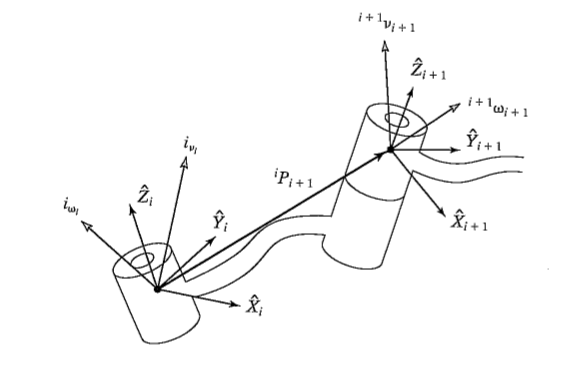
\includegraphics[width=.8\textwidth]{rigidbody/fig/velocity-transfer.png}
    \caption{Μετάδοση της ταχύτητας από άρθρωση σε άρθρωση\protect\footnotemark}
    \label{fig:velocity-transfer}
\end{figure}
\footnotetext{Εικόνα από το βιβλίο \cite{craig95}}

%%%%%%%%%%%%%%%%%%%%%%%%%%%%%%%%%%%%%%%%%%%%%%%%%%%%%%%%%%%%%%%%%%%%%%%%%%%%%%%%
\subsection{Αντίστροφη Κινηματική}

Η αντίστροφη κινηματική είναι ένα σημαντικό εργαλείο στα στάδια την διεξαγωγής του πειράματος. Με λίγα λόγια, είναι η διαδικασία που μετατρέπει τις θέσεις των αρθρώσεων στο καρτεσιανό τρισδιάστατο χώρο σε γενικευμένες συντεταγμένες του μοντέλου (γωνίες), έτσι ώστε κάθε χρονική στιγμή το μοντέλο να είναι στην ίδια διάταξη με τις μετρήσιμες θέσεις των αντίστοιχων αρθρώσεων. Παρακάτω θα δοθεί η μαθηματική διατύπωση για την λύση του προβλήματος και θα επισημανθούν κάποια λεπτά σημεία που ίσως οδηγήσουν σε λάθος αποτελέσματα.

Δοθέντος ενός συστήματος σωμάτων με $Ν$ βαθμών ελευθερίας με γενικευμένη συντεταγμένη $q^{t}_{j}$ και δοσμένη χρονική ακολουθία θέσεων για κάθε άρθρωση του μοντέλου $p^{t}_{j}$ με $j \in (1, N)$. Το πρόβλημα της εύρεσης των γενικευμένων συντεταγμένων για κάθε άρθρωση, ώστε να ελαχιστοποιηθεί το σφάλμα της απόστασης μεταξύ της παρατήρησης και της στάσης του μοντέλου, μπορεί να μοντελοποιηθεί σαν πρόβλημα βελτιστοποίησης \cite{sherman13}. Στόχος είναι η ελαχιστοποίηση του σφάλματος, όπου το σφάλμα είναι η αθροιστική συνάρτηση απόστασης μεταξύ του μοντέλου και των θέσεων. Σαν συνάρτηση απόστασης μπορεί να επιλεχθεί η Ευκλείδεια νόρμα 2ης τάξης. Επίσης κατά την επίλυση θα πρέπει να ληφθούν υπόψη και οι φυσικοί περιορισμοί της διάταξης για κάθε άρθρωση.

\begin{equation}
    \begin{aligned}
        & \underset{q_{j}}{\text{\eng{minimize}}}
        & & \sum_{i=1}^{N} w_{j} \cdot \norm{p_{j} - p(q_{j})}^{2} \\
        & \text{\eng{s.t.}}
        & & c_{j}(q_{j}) \leq b_{j}, \; i = 1, \ldots, N.
    \end{aligned}
    \label{equ:ik-optimization}
\end{equation}

Όπως φαίνεται στις εξισώσεις \ref{equ:ik-optimization}, οι $c_{j}(q_{j}) \leq b_{j}$ είναι οι περιορισμοί των αρθρώσεων. Που σημαίνει ότι η λύση των \eng{q's} θα πρέπει να την ικανοποιούν. Το $w_{j}$ είναι ο συντελεστής βαρύτητας για την συγκεκριμένη άρθρωση και καθορίζει πόσο σημαντική είναι στον υπολογισμό του σφάλματος.

Προβλήματα που μπορούν να εμφανιστούν κατά την διαδικασία είναι η πολλαπλή λύση όπως φαίνεται στην εικόνα \ref{fig:ik-multiple-solutions}. Αυτό οφείλεται στο αριθμό των βαθμών ελευθερίας, που αν είναι πολλοί τότε δίνουν ευελιξία στην διάταξη. Τρόποι που μπορούν να βελτιώσουν το αποτέλεσμα είναι η ελαχιστοποίηση των βαθμών ελευθερίας της διάταξης ή να εισαχθούν κατάλληλοι περιορισμοί. Για παράδειγμα, σε αρθρώσεις που έχουν τρεις βαθμούς ελευθερίας, όπως είναι ο γοφός, υπάρχει μεγάλη ευελιξία με αποτέλεσμα να δοθούν πολλαπλές λύσεις και να μην προσανατολιστεί σωστά το τμήμα του μηρού.

\begin{figure}[H]
    \centering
    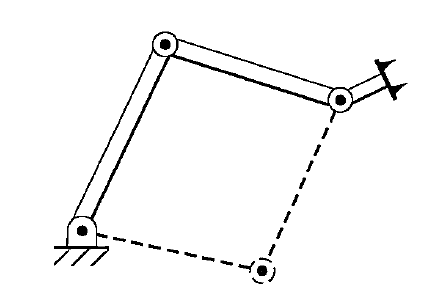
\includegraphics[width=.7\textwidth, height=.29\textheight]{rigidbody/fig/ik-multiple-solutions.png}
    \caption{Πολλαπλότητα λύσεων\protect\footnotemark}
    \label{fig:ik-multiple-solutions}
\end{figure}
\footnotetext{Εικόνα από το βιβλίο \cite{craig95}}

Ένα σημαντικό πρόβλημα που έχει να κάνει με τις δυνατότητες του συγκεκριμένου συστήματος καταγραφής, είναι ότι η πληροφορία που σου παρέχει μπορεί να μην αρκεί για να περιγράψει σωστά την διάταξη. Δηλαδή, αν υποθέσουμε ότι έχουμε μια άρθρωση με έξι βαθμούς ελευθερίας (τρεις περιστροφές και τρεις μετατοπίσεις), τότε για να επιλυθεί το σύστημα απαιτούνται τουλάχιστον τρία σημεία πάνω στο τμήμα, που να μην είναι συγγραμμικά μεταξύ τους. Για αυτό το λόγο, τα καλά συστήματα, όπως είναι το \eng{Vicon}, καταγράφουν πολλαπλές θέσεις σε κάθε τμήμα του σώματος.

%%%%%%%%%%%%%%%%%%%%%%%%%%%%%%%%%%%%%%%%%%%%%%%%%%%%%%%%%%%%%%%%%%%%%%%%%%%%%%%%
\section{Δυναμική}

Αφού έχει γίνει η ανάλυση της κινηματικής μπορεί κανείς να κάνει ένα βήμα πιο πέρα και να εξάγει σημαντικά συμπεράσματα για το μοντέλο, όπως είναι οι δυνάμεις και οι ροπές που ασκούνται στις αρθρώσεις για την παραγωγή της δοσμένης κίνησης. Η δυναμική είναι η μελέτη του υπολογισμού των δυνάμεων και των ροπών για δεδομένες τροχιές, ταχύτητες και επιταχύνσεις με βάση τον δεύτερο νόμο του Νεύτωνα.

Υπάρχουν διάφοροι μέθοδοι για τον υπολογισμό των δυνάμεων και των ροπών. Μια κατηγορία είναι η αναλυτική μέθοδος, η οποία σου δίνει όλη την πληροφορία της διάταξης. Οι πράξεις που απαιτούνται για τον υπολογισμό μιας χρονικής στιγμής όσον αφορά της προσθέσεις και τους πολλαπλασιασμούς είναι της τάξεως $O(n^4)$, όπου $n$ οι βαθμοί ελευθερίας της διάταξης. Από την άλλη έχουμε αναδρομικές μεθόδους, όπως είναι η \eng{Iterative Newton-Euler}, που είναι πιο αποδοτικές και επιτυγχάνουν πολυπλοκότητα της τάξεως $O(n)$.

Σκοπός όλων των μεθόδων είναι η επίλυση της γενικευμένης δυναμικής εξίσωσης \ref{equ:dynamics-equation} που περιγράφει την διάταξη.

\begin{equation}
    M(q) \cdot \ddot{q} + V(q, \dot{q}) + G(q) + F(q, \dot{q}) = \tau
    \label{equ:dynamics-equation}
\end{equation}

Όπου $q$ είναι η γενικευμένη συντεταγμένη των αρθρώσεων και είναι ένα διάνυσμα στήλης μεγέθους $n \times 1$, όσο είναι οι βαθμοί ελευθερίας του συστήματος. Ο $M(q)$ είναι ο πίνακας αδράνειας του συστήματος διαστάσεων $n \times n$ και εξαρτάται από το $q$ (την γενικευμένη θέση). Το διάνυσμα στήλης $V(q, \dot{q})$ μεγέθους $n \times 1$ συμβολίζει τις φυγόκεντρες δυνάμεις και τις δυνάμεις \eng{Coriolis}, που εξαρτιούνται από το τετράγωνο της ταχύτητας και του γινομένου των συζευγμένων ταχυτήτων αντίστοιχα. Το διάνυσμα στήλης $G(q)$ μεγέθους $n \times 1$ είναι η βαρύτητα που δρα πάνω στα διάφορα τμήματα της διάταξης. Το διάνυσμα $F(q, \dot{q})$ μεγέθους $n \times 1$ έχει να κάνει με τις εξωτερικές δυνάμεις, όπως είναι οι τριβές για παράδειγμα. Τέλος, από την άλλη μεριά της εξίσωσης έχουμε τις γενικευμένες δυνάμεις και ροπές που πρέπει να ασκηθούν στις αρθρώσεις για να παραχθεί η κίνηση και έχει διαστάσεις $n \times 1$.

%%%%%%%%%%%%%%%%%%%%%%%%%%%%%%%%%%%%%%%%%%%%%%%%%%%%%%%%%%%%%%%%%%%%%%%%%%%%%%%%
\subsection{Επίλυση με τον Αναδρομικό Αλγόριθμο}

Η περιγραφή των εξισώσεων του αλγορίθμου \eng{Iterative Newton-Euler} προϋποθέτουν την γνώση των θέσεων, των ταχυτήτων και των επιταχύνσεων $(q, \dot{q}, \ddot{q})$ για όλες τις αρθρώσεις. Επίσης, είναι απαραίτητη η γνώση της κατανομής της μάζας των τμημάτων του μοντέλου που υπολογίζονται ως προς το κέντρο μάζας. Ο αλγόριθμος αποτελείται από δύο βήματα. Το πρώτο βήμα, ξεκινώντας από την βάση μέχρι την άκρη (τελευταία άρθρωση στην αλυσίδα) του μοντέλου υπολογίζει τις ταχύτητες και τις επιταχύνσεις που διαδίδονται, αλλά και τις δυνάμεις και τις ροπές του κέντρου μάζας με βάση των εξισώσεων \ref{equ:iterative-NE-first}. Το δεύτερο βήμα, ξεκινώντας ανάποδα από την άκρη μέχρι την βάση υπολογίζει τις δυνάμεις και τις ροπές στις αρθρώσεις με βάση των εξισώσεων \ref{equ:iterative-NE-second}.

\begin{figure}[H]
    \centering
    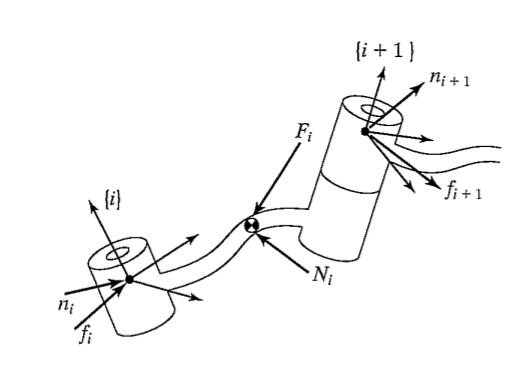
\includegraphics[width=.7\textwidth]{rigidbody/fig/force-balance.png}
    \caption{Διάγραμμα ελευθέρου σώματος\protect\footnotemark}
    \label{fig:force-balance}
\end{figure}
\footnotetext{Εικόνα από το βιβλίο \cite{craig95}}

Η πρώτη αναδρομή περιγράφεται από τις εξής σχέσεις για $i : 0 \rightarrow n-1$:

\begin{equation}
    \begin{aligned}
        ^{i+1}\omega_{i+1} = {}^{i+1}R_i \cdot {}^i\omega_i +
        \dot{q}_{i+1} \times {}^{i+1}\hat{Z}_{i+1}\\[10pt]
        ^{i+1}\dot{\omega}_{i+1} = {}^{i+1}R_i \cdot {}^i\dot{\omega}_i +
        {}^{i+1}R_i \cdot {}^i\omega_i \times \dot{q}_{i+1} \cdot
        {}^{i+1}\hat{Z}_{i+1} + \ddot{q}_{i+1} \cdot
        {}^{i+1}\hat{Z}_{i+1}\\[10pt]
        ^{i+1}\dot{u}_{i+1} = {}^{i+1}R_i \cdot (^i\dot{\omega}_i \times
        {}^iP_{i+1} + {}^i\omega_i \times (^i\omega_i \times {}^iP_{i+1}) +
        {}^i\dot{u}_i)\\[10pt]
        ^{i+1}\dot{u}_{C_{i+1}} = {}^{i+1}\dot{\omega}_{i+1} \times
        {}^{i+1}P_{C_{i+1}} + {}^{i+1}\omega_{i+1} \times (^{i+1}\omega_{i+1}
        \times {}^{i+1}P_{C_{i+1}}) + {}^{i+1}\dot{u}_{i+1}\\[10pt]
        ^{i+1}F_{i+1} = m_{i+1} \cdot {}^{i+1}\dot{u}_{C_{i+1}}\\[10pt]
        ^{i+1}N_{i+1} = {}^{C_{i+1}}I_{i+1} \cdot {}^{i+1}\dot{\omega}_{i+1} +
        {}^{i+1}\omega_{i+1} \times {}^{C_{i+1}}I_{i+1} \cdot {}^{i+1}\omega_{i+1}
    \end{aligned}
    \label{equ:iterative-NE-first}
\end{equation}

Η δεύτερη αναδρομή περιγράφεται από τις εξής σχέσεις για $i : n \rightarrow 1$:

\begin{equation}
    \begin{aligned}
        ^if_i = {}^{i}R_{i+1} \cdot {}^{i+1}f_{i+1} + {}^iF_i\\[10pt]
        ^in_i = {}^iN_i + {}^iR_{i+1} \cdot {}^{i+1}n_{i+1} + {}^iP_{C_i} \times
        {}^iF_i + {}^iP_{i+1} \times {}^iR_{i+1} \cdot {}^{i+1}f_{i+1}\\[10pt]
        \tau_i = {}^in^T_i \cdot {}^i\hat{Z}_i
    \end{aligned}
    \label{equ:iterative-NE-second}
\end{equation}

%%%%%%%%%%%%%%%%%%%%%%%%%%%%%%%%%%%%%%%%%%%%%%%%%%%%%%%%%%%%%%%%%%%%%%%%%%%%%%%%
\subsection{Αντίστροφη Δυναμική}

Το πρόβλημα της αντίστροφης δυναμικής ορίζεται ως την έρευνα των γενικευμένων ροπών ή δυνάμεων που πρέπει να ασκηθούν στις αρθρώσεις, ώστε το σύστημα να παράξει την συγκεκριμένη κίνηση. Κοιτάζοντας την εξίσωση \ref{equ:dynamics-equation} ουσιαστικά ο άγνωστος είναι το $\tau $ σε κάθε χρονική στιγμή της εξέλιξης της κίνησης. Είναι φανερό ότι απαιτείται η γνώση των υπόλοιπων παραμέτρων που βρίσκονται αριστερά της εξίσωσης. Συνήθως η διαδικασία της αντίστροφης δυναμικής βασίζεται στα αποτελέσματα της αντίστροφης κινηματικής που προσδιορίζει μια ακολουθία από \eng{q's}. Είναι απαραίτητο να εξαχθούν και οι άλλες δύο παράγωγοι $(\dot{q}, \ddot{q})$ με την βοήθεια αριθμητικών παραγώγων.

Πρέπει να επισημάνουμε την σημασία των εξωτερικών δυνάμεων στον υπολογισμό του $\tau $ στην εξίσωση. Επίσης οι προσεγγίσεις που κάνουμε στην μοντελοποίηση σε συνδυασμό με τα σφάλματα που εισάγονται από τις προσεγγίσεις των παραγώγων, λαμβάνουν μεγάλο ρόλο στην ακρίβεια των λύσεων. Τέλος, η προσέγγιση της αδράνειας του συστήματος είναι σημαντικός παράγοντας στην ανάλυση και ταυτόχρονα είναι πολύ δύσκολο να εκτιμηθεί.

%%%%%%%%%%%%%%%%%%%%%%%%%%%%%%%%%%%%%%%%%%%%%%%%%%%%%%%%%%%%%%%%%%%%%%%%%%%%%%%%
\subsection{Ορθή Δυναμική}

Γενικά η διαδικασία της ορθής κινηματικής είναι ευαίσθητη σε σφάλματα και μπαίνει πολύ εύκολα σε αστάθεια. Δεδομένου των γενικευμένων δυνάμεων και ροπών που ασκούνται στο σύστημα σκοπός είναι να βρεθούν οι γενικευμένες συντεταγμένες \eng{q's} και να παραχθεί κίνηση. Λύνοντας την \ref{equ:dynamics-equation} ως προς τις επιταχύνεις καταλήγουμε στην εξίσωση \ref{equ:forward-dynamics}.

\begin{equation}
    \ddot{q} = M(q)^{-1} \cdot \{ \tau - V(q, \dot{q}) - G(q) - F(q, \dot{q})\}
    \label{equ:forward-dynamics}
\end{equation}

Αν ολοκληρώσουμε την επιτάχυνση δύο φορές με κάποια αριθμητική μέθοδο ολοκλήρωσης, λαμβάνουμε τις γενικευμένες συντεταγμένες \eng{q's}. Παρόλο που το πρόβλημα φαίνεται απλό στην πραγματικότητα αν τροφοδοτήσουμε το μοντέλο με τις υπολογισμένες τιμές των \eng{q's}, δεν θα παραχθεί σωστή κίνηση και πολύ πιθανό να μπει στην αστάθεια. Αυτό γιατί στην πραγματικότητα παραβιάζεται ο 2ος νόμος του Νεύτωνα $F \neq m \cdot a$, κυρίως λόγω σφαλμάτων που συσσωρεύονται κατά την διαδικασία.

Για να καταλάβουμε το πρόβλημα ας θυμηθούμε τι θα θέλαμε να κάνουμε. Αρχικά έγινε η καταγραφή μιας κίνησης και το αποτέλεσμα μαζί με ένα μοντέλο χρησιμοποιείται στην αντίστροφη κινηματική, για να παραχθούν οι γενικευμένες συντεταγμένες του μοντέλου. Παράλληλα έχουν καταγραφεί οι εξωτερικές δυνάμεις και έχει γίνει μια εκτίμηση των παραμέτρων αδράνειας. Με βάση το αποτέλεσμα της αντίστροφης κινηματικής αν παραγωγίσουμε δύο φορές την ακολουθία και τροφοδοτούμε την διαδικασία της αντίστροφης δυναμικής έτσι ώστε να μας να υπολογίσει τις γενικευμένες ροπές. Τέλος, χρησιμοποιούμε τις γενικευμένες ροπές και εκτελούμε ορθή δυναμική. Συμπερασματικά, α) έχουμε εισάγει θόρυβο από τις μετρήσεις των τροχιών και των εξωτερικών δυνάμεων, β) φτιάξαμε ένα μοντέλο που προσεγγίζει το δείγμα, γ) προσεγγίσαμε τις δύο παραγώγους από τις μετρήσεις με αριθμητικές μεθόδους εισάγοντας σφάλμα, δ) κατά την εκτέλεση της αντίστροφης κινηματικής συσσωρεύτηκαν σφάλματα λόγω περιορισμένης ακριβείας ε) κάναμε υποθέσεις για την κατανομή της μάζας του δείγματος και προσεγγίσαμε την αδράνεια και στ) εισήχθησαν σφάλματα κατά την εκτέλεση της ορθής δυναμικής.
